\label{section:a}
\section{Graphene}
Graphene is a monolayer of carbon atoms arranged in a honeycomb lattice that can be thought of as two interpenetrating triangular sublattices with two nonequivalent carbon atoms.
\begin{figure}[H]
	\centering
	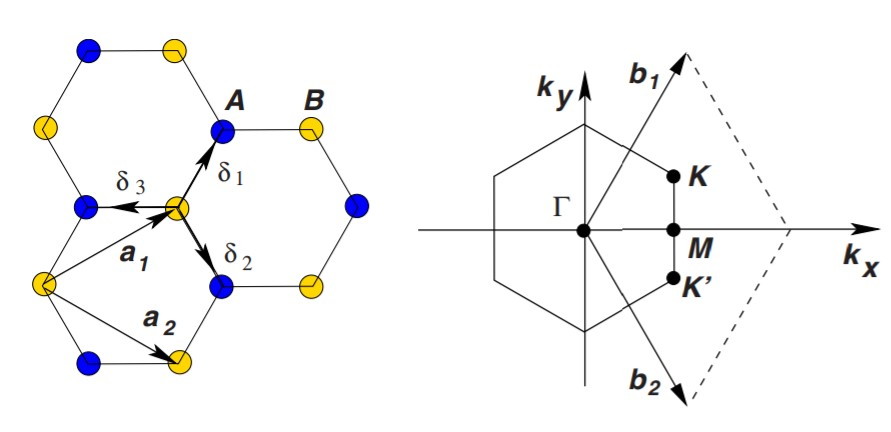
\includegraphics[width=\textwidth]{figures/lattice.jpg}
	\caption{Graphene Lattice and its Brillouin zone. Left: Two interpenetrating triangular lattices forming graphene honeycomb lattice. $a_1$ and $a_2$ are lattice vectors and $\delta_i, i=1,2,3$ are the nearest neighbour vectors. Right: Corresponding Brillouin zone that shows high symmetry points. The Dirac cones are located at $K$ and $K^\prime$ points. Figure adapted from \cite{Geim}}
	\label{fig:lattice}
\end{figure}
The primitive lattice vectors for the lattice are given by (see fig. \ref{fig:lattice}):
\begin{equation}
	a_1 = \frac{a}{2}(3,\sqrt{3}), a_2 = \frac{a}{2}(3,-\sqrt{3})
\end{equation}
The reciprocal lattice vectors are given by (see fig. \ref{fig:lattice}):
\begin{equation}
	b_1 = \frac{2\pi}{3a}(1,\sqrt{3}), b_2 = \frac{2\pi}{3a}(1,-\sqrt{3})
\end{equation}
The wave vectors of the high symmetry points in the first Brillouin zone are given below, where $K$ and $K^{\prime}$ are two nonequivalent corners known as the Dirac points, as shown in fig. \ref{fig:lattice}.
\begin{equation}
	\Gamma = (0,0),K=\frac{2\pi}{3a}(1,\frac{1}{\sqrt{3}}),K^{\prime}=\frac{2\pi}{3a}(1,-\frac{1}{\sqrt{3}}),M=\frac{2\pi}{3a}(1,0)
\end{equation}
The electronic structure of graphene can be derived using the tight binding model, considering nearest and next nearest neighbour hopping. The Hamiltonian becomes:
\begin{equation}
	H= -t\sum_{<i,j>,\sigma}(a_{\sigma,i}^\dagger b_{\sigma,j}+H.c)-t^\prime(a_{\sigma,i}^\dagger a_{\sigma,j}+b_{\sigma,i}^\dagger b_{\sigma,j}+H.c.)
\end{equation}
where $a_{\sigma,i}$, $a_{\sigma,i}^\dagger$ and $b_{\sigma,i}$, $b_{\sigma,i}^\dagger$ are the annihilation and creation operators on site A and B, with spin $\sigma$, respectively. $t$ is the nearest neighbour hopping energy $\approx 2.7eV$ and $t^\prime$ is the next nearest neighbour hopping energy $\approx -0.2 t$. We can diagonalise the Hamiltonian and derive the electronic dispersion to be \cite{Geim}:
\begin{equation}
	E_\pm(\mathbf{k})=\pm t \sqrt{f(\mathbf{k})+3}-t^\prime f(\mathbf{k}), f(\mathbf{k})= cos(\frac{\sqrt{3}}{2}k_y a)cos(\frac{3}{2}k_x a )+2cos(\sqrt{3}k_y a)
\end{equation}

\begin{figure}[H]
	\centering
	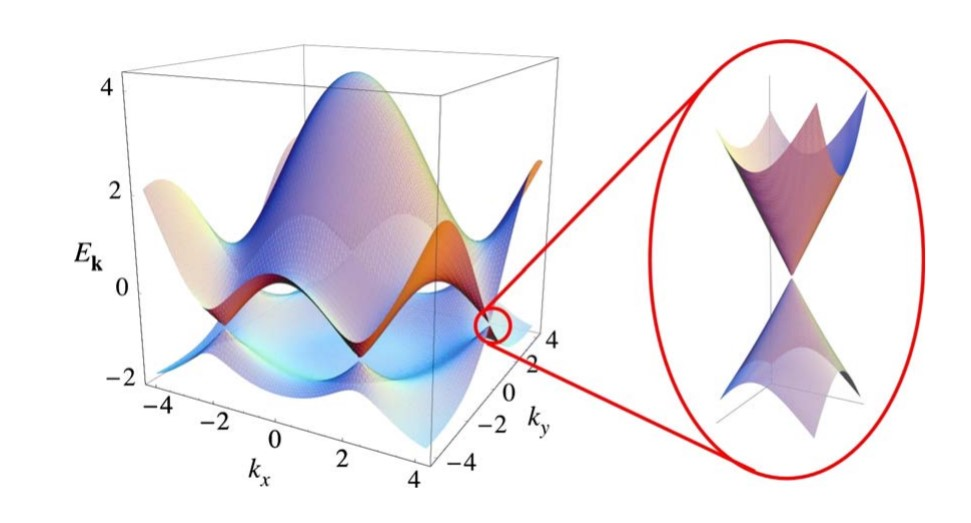
\includegraphics[width=\textwidth]{figures/dispersion.jpg}
	\caption{Electronic dispersion of graphene. Left: Energy spectrum of the honeycomb lattice in units of $t$ for non zero $t$ and $t^\prime$. Here $t=2.7 eV$ and $t^\prime=-0.2t$. Right: Zoom in of the energy bands near one of the Dirac points. Figure adapted from \cite{Geim}}
	\label{fig:dispersion}
\end{figure}
This gives a symmetric band structure for holes and electrons around zero energy, if we take $t^\prime$ to be zero. But the electron-hole symmetry is broken and the upper and lower bands become asymmetric for finite next nearest neighbour hopping. In
fig. \ref{fig:dispersion}, the full band structure of graphene is shown. A zoom in of the band structure close to one of the Dirac points is also shown. This dispersion can be
obtained by expanding the full band structure, close to $\mathbf{K}$ or $\mathbf{K^\prime}$ vector, i.e., $\mathbf{k}=\mathbf{K}+\mathbf{q}$ $(|\mathbf{q}|<<\mathbf{K})$:
\begin{equation}
	E_\pm(\mathbf{q})=\pm v_F|\mathbf{q}|+ O[(q/K)^2]
\end{equation}
where $\mathbf{q}$ is the momentum measured relatively to the
Dirac points and $v_F$ is the Fermi velocity, given by $v_F=3ta/ 2$.

The above equation shows that the energy bands linearly cross at the Dirac points, and hence the graphene acts as a zero band gap material with a linear dispersion. The approximation is valid for small carrier densities. From equation (2.6), the Hamiltonian near the Dirac points can be written as:
\begin{equation}
	H_{Dirac} =\begin{bmatrix}
		0 & q_x-i q_y \\
		q_x+i q_y & 0 
	\end{bmatrix} = v_F\mathbf{\sigma}.\mathbf{q}
\end{equation}
where $\sigma$ is the corresponding Pauli matrices. This is equivalent to the equation for massless chiral Dirac fermions in 2D where the speed of light has been replaced by $v_F$ and with a pseudospin spinor structure related to the graphene sublattices. Many of the interesting properties of graphene can be explained using this unique and interesting dispersion.

\section{Bilayer graphene}
\begin{figure}[H]
	\centering
	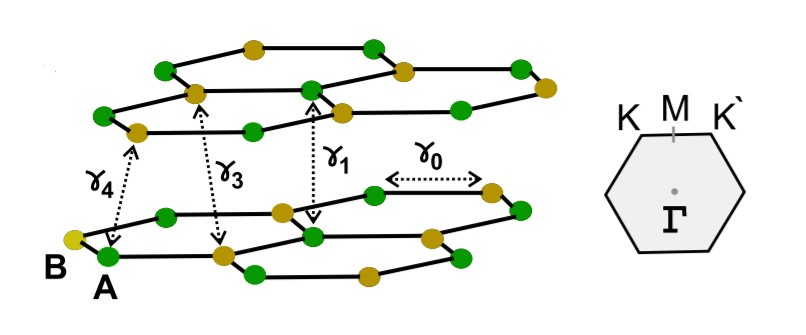
\includegraphics[width=\textwidth]{figures/bilayer_lattice.jpg}
	\caption{Bernal stack bilayer graphene lattice with hopping terms and its Brillouin zone. Left: Two monolayer graphene in AB stacking forming bernal stack bilayer graphene lattice. $\gamma_0$, $\gamma_1$, $\gamma_3$ and $\gamma_4$ are the hopping terms. Right: Corresponding Brillouin zone that shows high symmetry points. Figure adapted from \cite{Geim}}
	\label{fig:bilayer_lattice}
\end{figure}
Bilayer graphene usually refers to AB stacking or Bernal stacking in which two layers of graphene are stacked on top of each other such that the two layers are shifted by one atomic spacing, as shown in fig. \ref{fig:bilayer_lattice}. The tight binding model gives us the energy dispersion of bilayer graphene. Considering various hopping terms - in-plane nearest neighbour hopping, $\gamma_0\approx2.7 eV$, hopping between atom $A_1$ and atom  $A_2$, $\gamma_1\approx0.4$, hopping between atom $B_1$ and atom $B_2$, $\gamma_1\approx0.3$ and hopping between atom $A_1(A_2)$ and atom $B_2(B_1)$, the tight-binding Hamiltonian becomes:

\begin{align}
	\begin{split}
		H & = -\gamma_0\sum_{<i,j>,m,\sigma}(a_{i,m,\sigma}^\dagger b_{j,m,\sigma}+H.c.)-\gamma_1 \sum_{j,\sigma}(a_{j,1,\sigma}^\dagger a_{j,2,\sigma}+H.c.) \\
		& -\gamma_3 \sum_{j,\sigma}(b_{j,1,\sigma}^\dagger b_{j,2,\sigma}+H.c.)-\gamma_4 \sum_{j,\sigma}(a_{j,1,\sigma}^\dagger b_{j,2,\sigma}+a_{j,2,\sigma}^\dagger b_{j,1,\sigma}+H.c.)
	\end{split}
\end{align}
where $a_{i,m,\sigma}$($b_{j,m,\sigma}$) annhilates an electron on sublattice $A(B)$ with spin $\sigma$ on plane $m=1,2$. If we apply a perpendicular electric field to the system, an electrochemical potential $\Delta$ is added between the layers. The Hamiltonian in the $k$ space near the $K(K^\prime)$ points, ignoring the weaker hopping terms $\gamma_3$ and $\gamma_4$, can be represented as \cite{Geim}: 
\begin{equation}
	H_{K/K^\prime} = \begin{bmatrix}
		-\frac{\Delta}{2} & v_Fk & 0 & 0 \\
		v_Fk & -\frac{\Delta}{2} & \gamma_1 & 0 \\
		0 & \gamma_1 & \frac{\Delta}{2} & v_Fk \\
		0 & 0 & v_Fk & \frac{\Delta}{2}
	\end{bmatrix}
\end{equation}
The resultant electronic dispersion near the Dirac points is given by:
\begin{equation}
	E_\pm^2 = \frac{\Delta^2}{4}+v_F^2k^2+\frac{\gamma_1^2}{2}\pm\sqrt{\Delta^2v_F^2k^2+\gamma_1^2v_F^2k^2+\frac{\gamma_1^4}{4}}
\end{equation}
This equation gives rise to four solutions, hence, four bands near the $K(K^\prime)$ points, as shown in fig. \ref{fig:bilayer_dispersion}. For $\Delta=0$ and  $v_F<<\gamma_1$, the lowest two bands are given by:
\begin{equation}
	E\approx\frac{v_F^2k^2}{\gamma_1}
\end{equation}
We see that even bilayer graphene does not have a band gap when no external displacement field is applied. But unlike monolayer graphene which has a linear dispersion, bilayer graphene has a parabolic dispersion near the Dirac points, with effective mass $m^*=\frac{\gamma_1}{2v_F^2}$.
For $\Delta\neq 0$ and $\Delta<<\gamma_0$, the lowest two bands are given by:
\begin{equation}
	E \approx \frac{\Delta}{2}-\frac{ \Delta v^{2}_{F} k^{2}}{\gamma_1}+\frac{v^{4}_F k^{4}}{ \gamma_1^{2} \Delta}
\end{equation}
In the presence of a displacement field, we see that a band gap opens up, which can be tuned by changing the applied perpendicular electric field.

\begin{figure}[H]
	\centering
	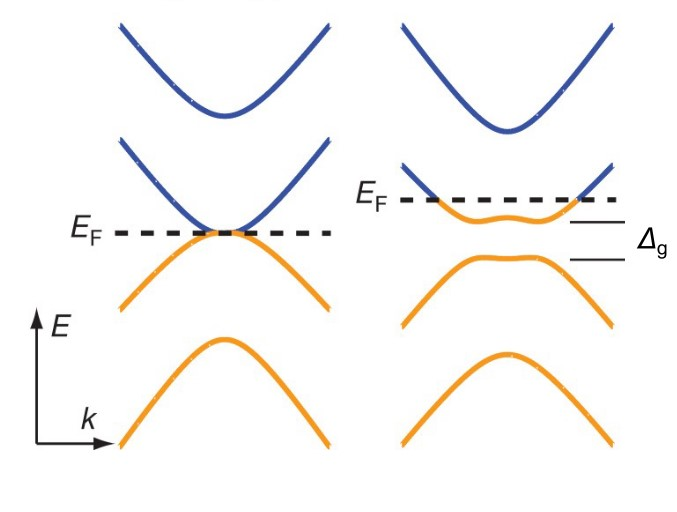
\includegraphics[width=0.6\textwidth]{figures/bilayer_dispersion.jpg}
	\caption{Electronic dispersion of bilayer graphene when $\Delta=0$ (left) and $\Delta\neq0$ (right). A band gap $\Delta_g$ opens up in the presence of an external displacement field. Figure adapted from \cite{Zhang2009}}
	\label{fig:bilayer_dispersion}
\end{figure}

\section{Twisted bilayer graphene}
\subsection{Moiré superlattices}
A geometric interference pattern, known as Moiré pattern, is formed when two-dimensional crystals with a lattice mismatch or a relative twist between them are stacked on top of each other. The wavelength of the Moiré pattern in case two layers of graphene is given by:
\begin{equation}
	\lambda = \frac{(1+\delta)a}{\sqrt{2(1+\delta)(1-cos\theta)+\delta^2}}
\end{equation}
where $a$ is the lattice constant of graphene, $\theta$ is the twist angle between the two layers and $\delta$ is the lattice mismatch between the two layers. Moiré pattern gives rise to effective superlattice potential with a periodicity different from the original lattice. We can see that the Moiré wavelength becomes much larger than the lattice constant for small twist angles. When $\lambda$ becomes comparable to the Fermi wavelength, the electronic structure is significantly modified. For example, aligned graphene-hBN heterostructures give rise to secondary Dirac points as a result of the Moiré superlattice potential.

In case of twBLG, the twist between the graphene layers gives rise to formation of a Moiré superlattice and creation of mini Brillouin zone, as shown in fig. \ref{fig:twblg_lattice}. The mini Brillouin zone can be constructed from the difference between the two $K(K^\prime)$ wavevectors for the two layers. Band structure is changed with formation of flat bands with high density of states, which we discuss in the following sections.

\begin{figure}[H]
	\centering
	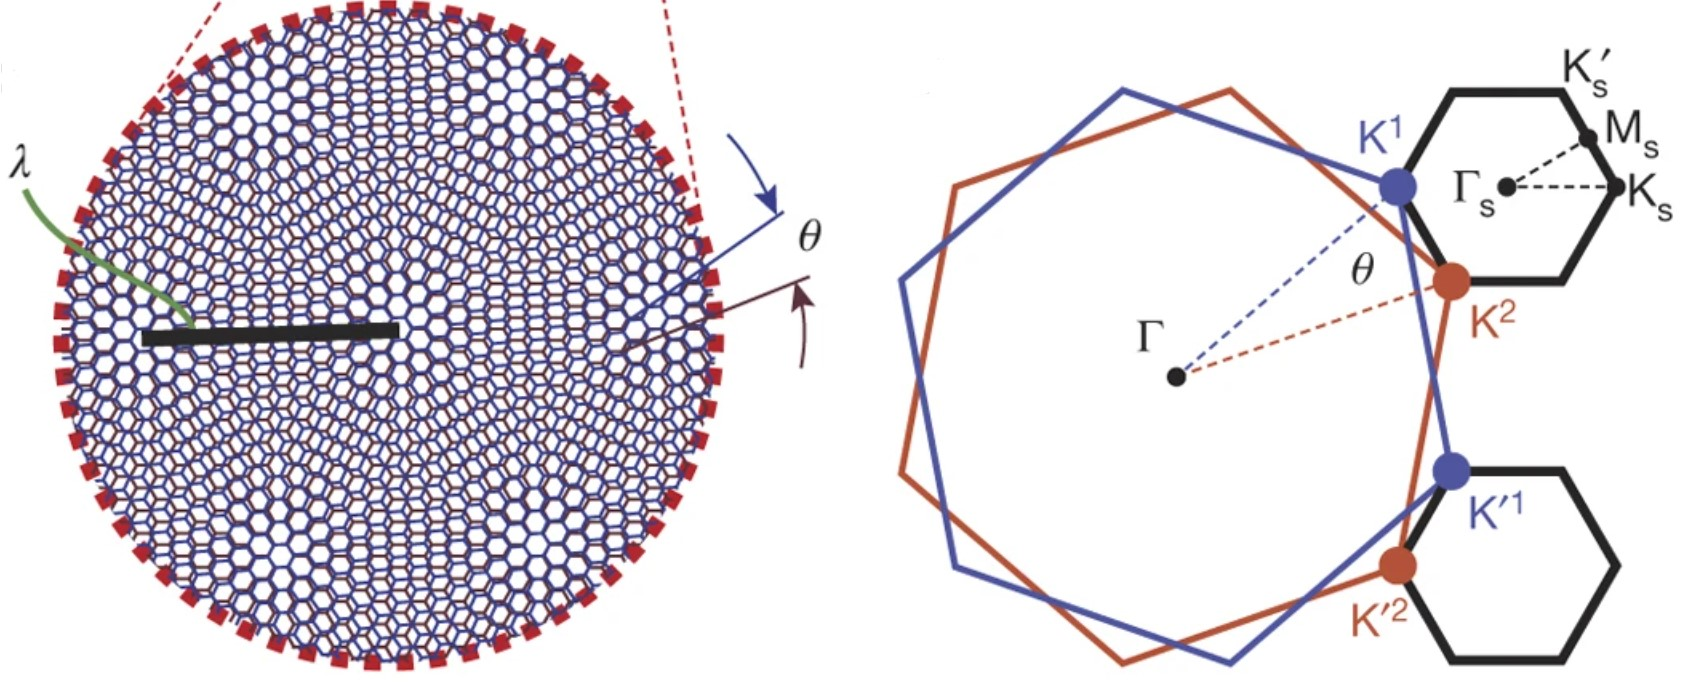
\includegraphics[width=\textwidth]{figures/twblg_lattice.jpg}
	\caption{twBLG Moiré pattern and its mini Brillouin zone. Left:  The Moiré pattern as seen in twBLG. The Moiré wavelength is $\lambda=\frac{a}{2sin(\theta/2)}$. Right: The mini Brillouin zone is constructed from the difference between the two $K(K^\prime)$ wavevectors for the two layers. $K_s$,$K_s^\prime$,$M_s$ and $\Gamma_s$ denote points in the mini Brillouin zone. Figure adapted from \cite{Cao2018}}
	\label{fig:twblg_lattice}
\end{figure}

\subsection{Continuum model developed by MacDonald}
The geometry of the bilayer system is characterised by a twist angle $\theta$ and a translation vector $\mathbf{d}$. But commensurability is determined only by the twist angle. We will discuss continuum model developed by MacDonald. \cite{Bistritzer12233} In a commensurate structure, sliding one layer with respect to another modifies the unit cell but leaves the bilayer crystalline. So, let's consider AB stacking as the aligned configuration. The positions of the carbon atoms in the two layers are then $\mathbf{R}$ and $\mathbf{R^{\prime}} = M(\theta)(\mathbf{R}-\tau)+\mathbf{d}$, where $\tau$ is a vector connecting the two atoms in the unit cell, and $M$ is a two dimensional rotation matrix within the graphene plane.

The bilayer forms a two-dimensional crystal only at a discrete set of commensurate twist angles. Bloch's theorem doesn't apply microscopically at generic twist angles and hence direct electronic structure calculations are not possible. For twist angles larger than a few degrees, except for a small set of angles that give low-order commensurate structure, the two layers are electronically isolated. As the twist angle reduces, interlayer coupling strengthens and quasiparticle velocity at Dirac point decreases. They derive a low-energy effective Hamiltonian valid for any value of $\mathbf{d}$ and for small twist angles, $\theta<10^o$. \cite{Bistritzer12233}
\begin{figure}[H]
	\centering
	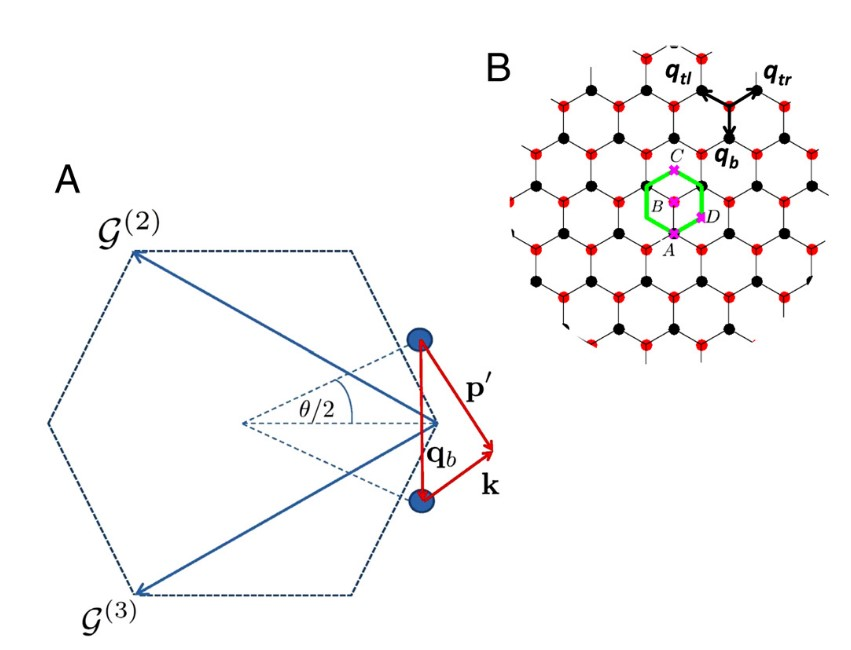
\includegraphics[width=\textwidth]{figures/contmodel.jpg}
	\caption{twBLG in momentum space (A) Dashed line marks the first Brillouin zone of an unrotated layer. The three equivalent Dirac points are connected by  $\mathcal{G}^{(2)}$ and $\mathcal{G}^{(3)}$. The circles represent Dirac points of the rotated graphene layers, separated by $k_\theta = 2k_D sin(\theta/2)$, where $k_D$ is the magnitude of the Brillouin-zone corner wave vector for a single layer. (B) The three equivalent Dirac points in the first Brillouin zone result in three distinct hopping processes. For all the three processes $|q_j| = k_\theta$. The green solid line marks the Moiré band Wigner–Seitz cell. The red and black circles mark the Dirac points of the two layers. Figure adapted from \cite{Bistritzer12233}}
	\label{fig:contmodel}
\end{figure}
The low-energy continuum model Hamiltonian has three terms: two single-layer Dirac-Hamiltonian terms that are associated with the isolated graphene sheets and a tunneling term that accounts for the hopping between the layers. The Dirac-Hamiltonian for a layer rotated by an angle $\theta$ with respect to a fixed coordinate system is given by \cite{Geim}:
\begin{equation}
	h_{\mathbf{k}}(\theta)=-vk \begin{bmatrix}
		0 & e^{i(\theta_{\mathbf{k}}-\theta)}\\
		e^{-i(\theta_{\mathbf{k}}-\theta)} & 0 
	\end{bmatrix}
\end{equation}
where $\mathbf{k}$ is the momentum measured from the Dirac point, $v$ is the Dirac velocity, $\theta_{\mathbf{k}}$ is the momentum orientation relative to the x axis. Choosing the coordinate system as shown in fig. \ref{fig:contmodel}, the decoupled bilayer Hamiltonian is $\ket{1} h(\theta/2)\bra{1}+\ket{2}h(-\theta/2)\bra{2}$, where $\bra{i}\ket{i}$ projects onto layer $i$.

Assuming that the interlayer tunneling amplitude between the $\pi$-orbitals is a smooth function of spatial separation projected onto the graphene planes, a continuum model is derived. The matrix element,
\begin{equation}
	T_{\mathbf{kp^\prime}}^{\alpha\beta}=\bra{\Psi_{\mathbf{k}\alpha}^{(1)}}H_T\ket{\Psi_{\mathbf{p\prime}\beta}^{(2)}}
\end{equation}
of the tunneling Hamiltonian $H_T$, describes a process in which an electron with momentum $\mathbf{p\prime}=M\mathbf{p}$ on sublattice $\beta$ in one layer hops to a momentum $\mathbf{k}$ on sublattice $\alpha$ in the other layer.

In a $pi$-band tight-binding model the projection of the wavefunctions of the two layers onto a given sublattice are:
\begin{equation}
	\ket{\psi_{\mathbf{k} \alpha}^{(1)}}=\frac{1}{\sqrt{N}} \sum_{\mathbf{R}} e^{i \mathbf{k}\left(R+\tau_{\alpha}\right)}\ket{\mathbf{R}+\tau_{\alpha}}
\end{equation}
and
\begin{equation}
	\ket{\psi_{\mathbf{p} \beta}^{(2)}}=\frac{1}{\sqrt{N}} \sum_{\mathbf{R}^{\prime}} e^{i \mathbf{p}\left(R^{\prime}+\tau_{\beta}^{\prime}\right)}\ket{\mathbf{R}^{\prime}+\tau_{\beta}^{\prime}}
\end{equation}
In this case, $\tau_{\alpha}=0$, $\tau_{\beta}=\tau$, and $\mathbf{R}$ is summed over the triangular Bravais lattice. Using the above equations and the two-center approximation,
\begin{equation}
	\mel{\mathbf{R}+\tau_{\alpha}}{H_T}{\mathbf{R}^\prime +\tau_{\beta}^\prime}=t(\mathbf{R}+\tau_{\alpha}-\mathbf{R}^\prime - \tau_{\beta}^\prime)
\end{equation}
for the interlayer hopping amplitude in which $t$ depends on the difference between the positions of the two carbon atoms. It is found that
\begin{equation}
	T_{\mathbf{k p}^{\prime}}^{\alpha \beta}=\sum_{\mathbf{G}_{1} \mathbf{G}_{2}} \frac{t_{\overline{\mathbf{k}}+\mathbf{G}_{1}}}{\Omega} e^{i\left[\mathbf{G}_{1} \tau_{\alpha}-\mathbf{G}_{2}\left(\tau_{\beta}-\tau\right)-\mathbf{G}_{2}^{\prime} \mathbf{d}\right]} \delta_{\overline{\mathbf{k}}+\mathbf{G}_{1}, \overline{\mathbf{p}}^{\prime}+\mathbf{G}_{2}^{\prime}}
\end{equation}
where, $\Omega$ is the unit cell area, $t_{\mathbf{q}}$ is the Fourier transform of the tunneling amplitude $t(\mathbf{r})$, the vectors $\mathbf{G_1}$ and $\mathbf{G_2}$ are summed over reciprocal lattice vectors, and $\mathbf{G_2}^\prime = M \mathbf{G_2}$. Here, momentum is measured relative to the center of the Brillouin zone and not relative to the Dirac point.

The continuum model for $H_T$ is obtained by measuring wave vectors in both layers relative to their Dirac points and assuming that the deviations are small compared to Brillouin-zone dimensions. Although $t_q$ is not precisely known, it should fall to zero very rapidly with $q$ on the reciprocal lattice vector scale. This is because the graphene layer separation exceeds the separation between carbon atoms in a layer by more than twice.

The largest $t_q$ values that enter the tunneling near the Dirac point have $q=k_D$, the Brillouin-zone corner (Dirac) wave vector magnitude, and correspond to the three reciprocal vectors $\mathbf{0}$, $\mathcal{G}^{(2)}$, and $\mathcal{G}^{(3)}$ where the latter two vectors connect a Dirac point with its equivalent first Brillouin-zone counterparts (See fig. \ref{fig:contmodel}). When only these terms are retained,
\begin{equation}
	T^{\alpha \beta}(\mathbf{r})=w \sum_{j=1}^{3} \exp \left(-i \mathbf{q}_{j} \cdot \mathbf{r}\right) T_{j}^{\alpha \beta}
\end{equation}
where $w=t_{k_D}/\Omega$ is the hopping energy,

\begin{equation}
	T_1 = \begin{bmatrix}
		1 & 1 \\
		1 & 1
	\end{bmatrix}, \; \;
	T_2=e^{-i \mathcal{G}^{(2)\prime} \cdot \mathbf{d}} \begin{bmatrix}
		e^{-i \phi} & 1 \\ e^{i \phi} & e^{-i \phi}
	\end{bmatrix}, \; \;
	T_3=e^{-i \mathcal{G}^{(3)\prime} \cdot \mathbf{d}} \begin{bmatrix}
		e^{i \phi} & 1 \\ e^{-i \phi} & e^{i \phi}
	\end{bmatrix}
\end{equation}
and $\phi=2/3$. The three $\mathbf{q}_j$’s are Dirac model momentum transfers that correspond to the three interlayer hopping processes. For $\mathbf{d}=0$ and a vanishing twist angle, the continuum tunneling matrix is $3w\delta_{\alpha A}\delta_{\beta B}$, independent of position.

\begin{figure}[H]
	\centering
	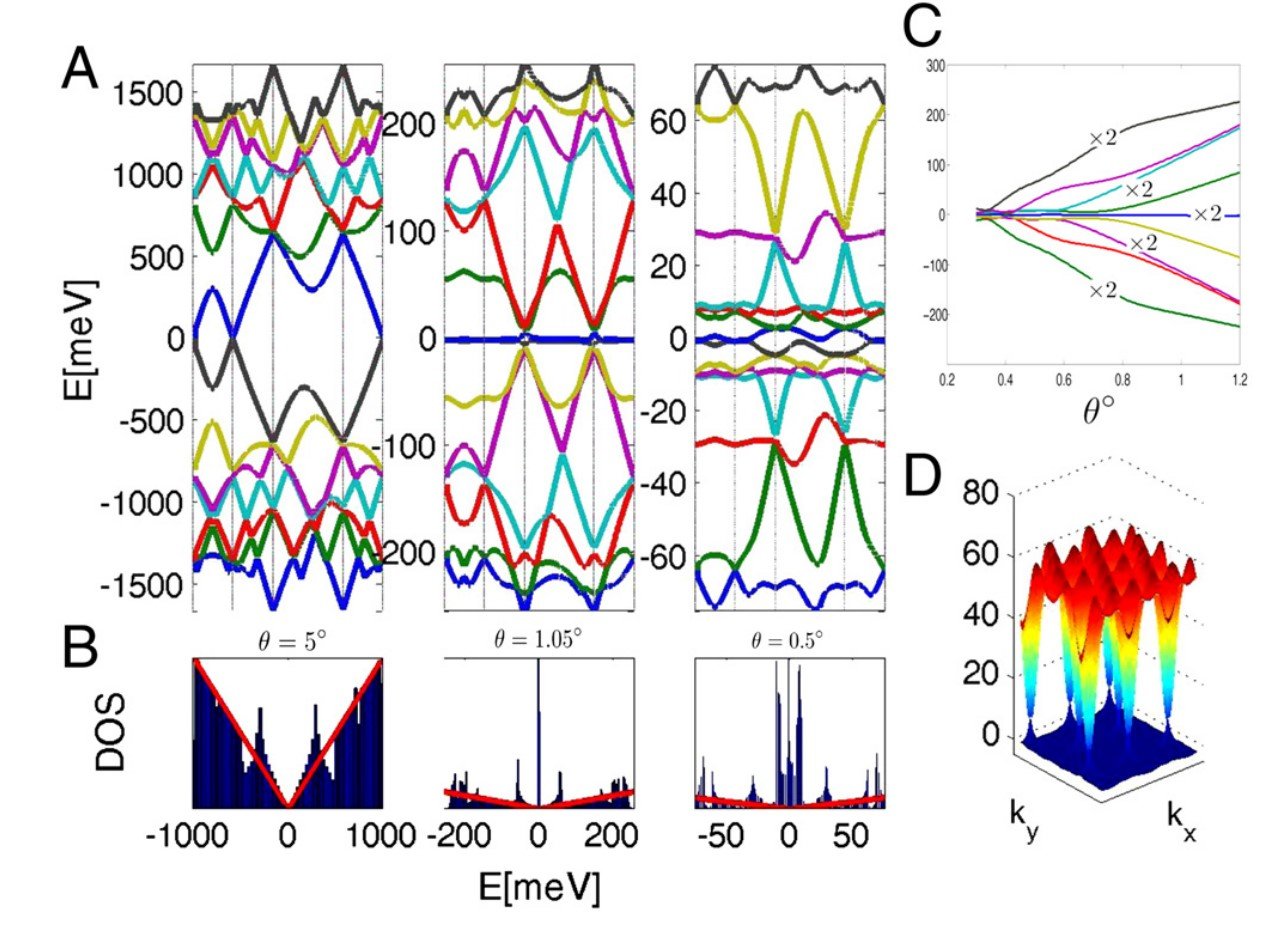
\includegraphics[width=\textwidth]{figures/contmodelband.jpg}
	\caption{Moiré bands (A) Energy dispersion plotted along A-B-C-D-A (see fig. \ref{fig:contmodel}), for bands closest to the Dirac point. (B) Density of states. (C)  Energy as a function of twist angle for the $k=0$ states. (D) Full dispersion of the flat band at $\theta = 1.05^o$. Figure adapted from \cite{Bistritzer12233}}
	\label{fig:contmodelband}
\end{figure}

In the continuum model, hopping is local and periodic, allowing Bloch’s theorem to be applied at any rotation angle irrespective of whether or not the bilayer is crystalline. Solving the Moiré bands numerically using the plane wave expansion illustrated in fig. \ref{fig:contmodel}, convergence is attained by truncating momentum space at lattice vectors of the order of $w/\hbar v$. 

Up to a scale factor, the Moiré bands depend on a single parameter, $\alpha=w/vk_\theta$. Evaluating the Moiré bands as a function of their Brillouin-zone momentum $\mathbf{k}$ for different twist angles gives the result shown in fig. \ref{fig:contmodelband}. For large twist angles, the low-energy spectrum is virtually identical to that of an isolated graphene sheet, except that the velocity is slightly renormalised. Large interlayer coupling effects appear only near the high energy van Hove singularities discussed in \cite{Li2010}.

As the twist angle is reduced, the number of bands in a given energy window increases and the band at the Dirac point narrows. As illustrated in fig. \ref{fig:contmodelband}, it is seen that the Dirac-point velocity vanishes at $\theta \approx 1.05^o$, and that the vanishing velocity is accompanied by a very flat Moiré band which contributes a sharp peak to the Dirac-point density-of-states (DOS). At smaller twists, the Dirac-point velocity has a nonmonotonic dependence on twist angle, repeatedly vanishing at the series of magic angles illustrated in fig. \ref{fig:contmodelvel}.

\begin{figure}[H]
	\centering
	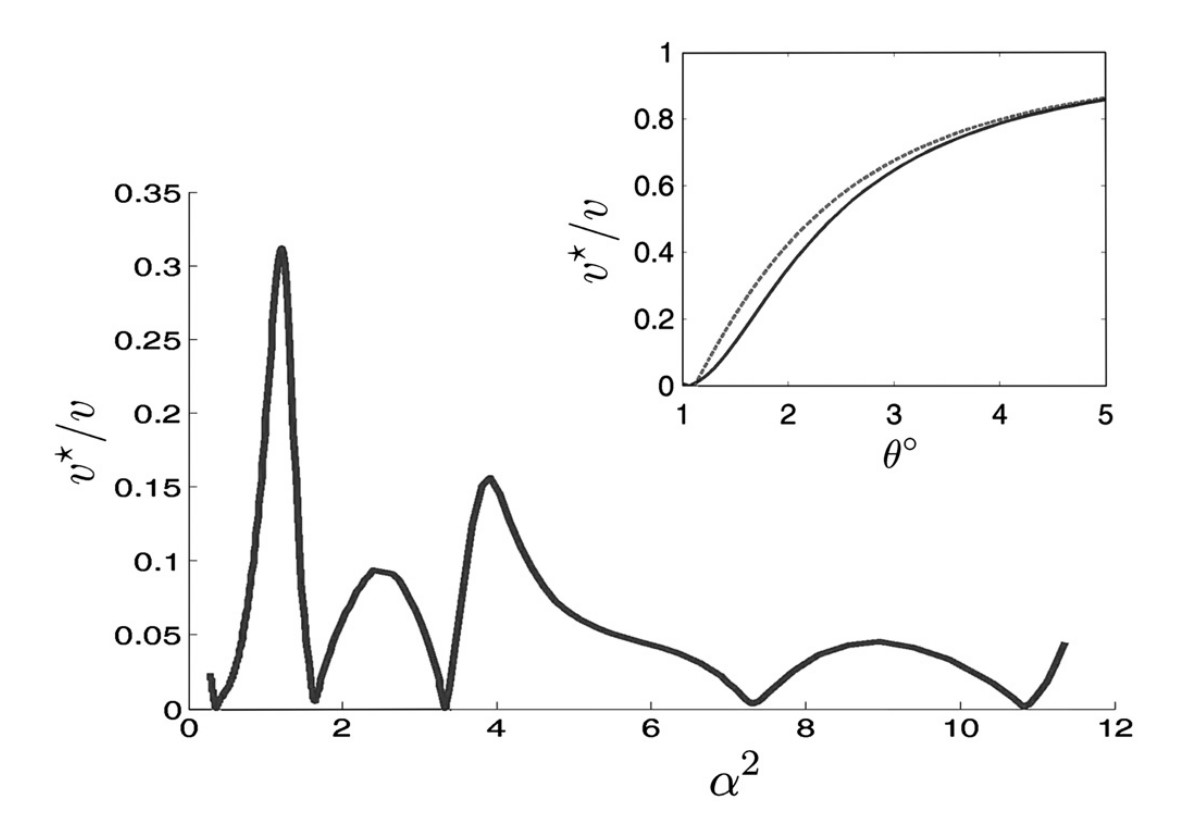
\includegraphics[width=0.7\textwidth]{figures/contmodelvel.jpg}
	\caption{Renormalized Dirac-point band velocity. The band velocity of the twBLG at the Dirac point plotted against $\alpha^2$, where $\alpha=w/vk_\theta$. Inset shows renormalised velocity at large twist angles. Figure adapted from \cite{Bistritzer12233}}
	\label{fig:contmodelvel}
\end{figure}

\subsection{Flat bands in twBLG}
Two graphene layers twisted at an angle with respect to each other gives rise to the formation of a mini Brillouin zone (BZ). The twist angle $\theta$ displaces the individual monolayer Dirac points by a wave-vector $|k_\theta|=2|K|sin(\theta/2)$, hence forming the mini BZ.

There is hybridisation of the Moiré bands leading to gap openings at the intersection of the Dirac cones and renormalisation of the Fermi velocity due to the interlayer coupling between the two graaphene layers. A series of magic angles, $\theta=1.05^o, 0.5^o, ...$ have been found at which the Fermi velocity at the Dirac points vanishes that gives rise to flat Moiré bands with large density of states. \cite{Bistritzer12233} The flat bands are formed as a result of competition between the interlayer hybridisation energy and the kinetic energy. When the hybridisation energy, $2w$, becomes comparable to the kinetic energy, $\hbar v_Fk_\theta$, the lower hybridised states are moved to zero energy leading to bands with very narrow band width (see fig. \ref{fig:flat}). \cite{Cao2018}
\begin{figure}[H]
	\centering
	\begin{subfigure}[b]{0.8\textwidth}
		\centering
		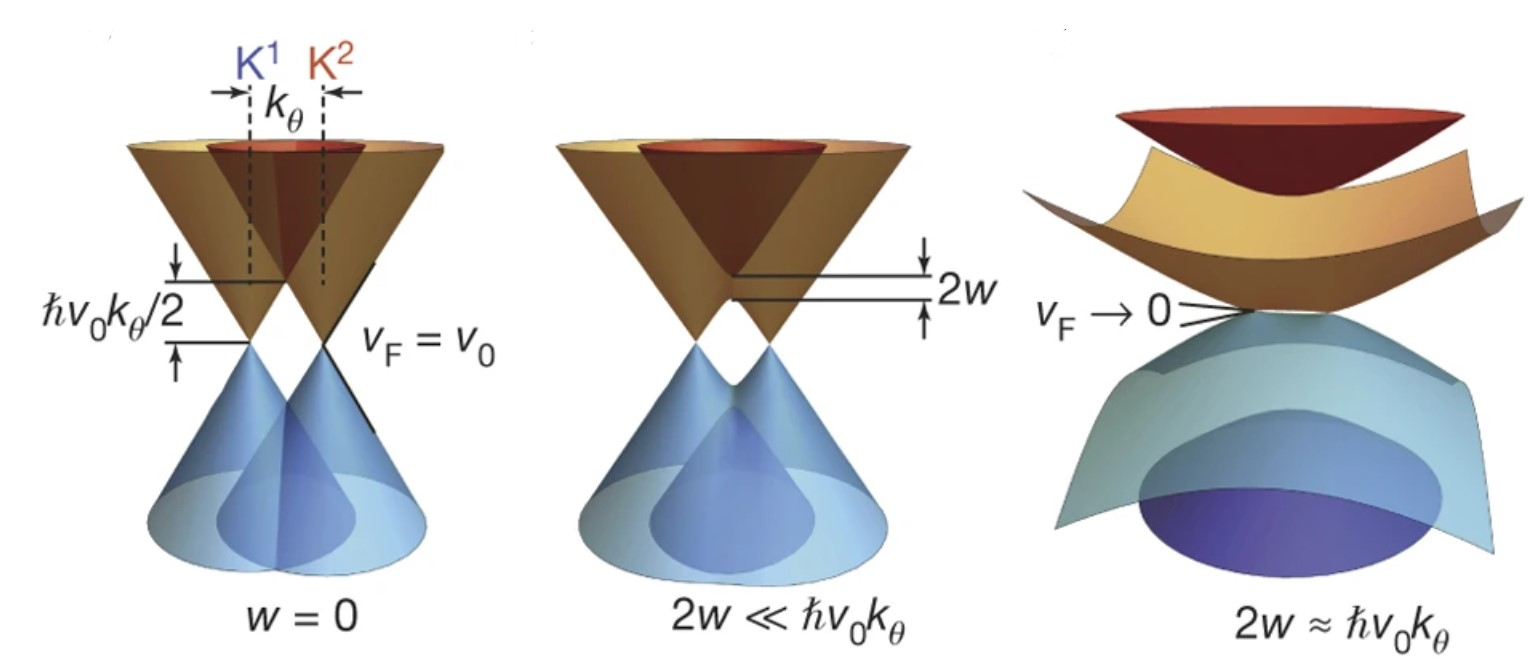
\includegraphics[width=\textwidth]{figures/twblg_hyb.jpg}
		\caption{Illustration of the effect of interlayer hybridization for $w=0$, $2w<<\hbar v_0 k_\theta$ and $2w\approx \hbar v_0 k_\theta$, where $v_0=10^6ms^{-1}$ is the Fermi velocity of graphene. Figure adapted from \cite{Cao2018}}
	\end{subfigure}
	
	\begin{subfigure}[b]{0.8\textwidth}
		\centering
		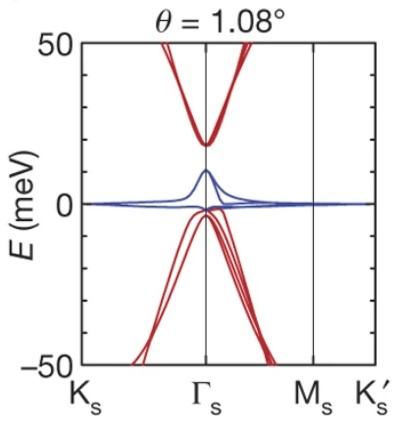
\includegraphics[width=0.5\textwidth]{figures/flatband.jpg}
		\caption{The band energy E of magic-angle ($\theta=1.08^o$) twBLG calculated using tight-binding method. The bands shown in blue are the flat bands. Figure adapted from \cite{Cao2018}}
	\end{subfigure}
	\caption{Electronic band structure of twBLG}
	\label{fig:flat}
\end{figure}

\subsection{Experimental signatures of twBLG}
\label{section:b}
The single-particle picture breaks down due to the presence of flat bands with large density of states near the charge neutrality point, because the Coulomb interactions exceed the kinetic energy in the system. twBLG enters various strongly correlated and topological states when the Fermi energy is tuned within the flat bands. It has been experimentally observed to show correlated insulating states,\cite{Cao2018} superconductivity,\cite{Cao2018_2} quantum anomalous Hall effect \cite{Serlin900,Wu2021}and ferromagnetism. \cite{Sharpe605}

Each Moiré superlattice band is four-fold degenerate at low twist angles. \cite{Cao2018} The charge density required to fill one superlattice band is given by:
\begin{equation}
	n_s=\frac{4}{A}=\frac{8\theta^2}{\sqrt{3}a^2}
\end{equation}
where $A$ is the area of the Moiré unit cell. The filling factor, $v=4n/n_s$ gives the number of electrons per Moiré unit cell.

Y. Cao and P. Jarillo-Herrero \textit{et al.} demonstrated a flat band nature of twBLG, that is evident from: (1) a reduced Fermi velocity, which is about 1/25 of that
in monolayer graphene, and (2) flattening of conductance minimum at the charge neutral point above 40 K. \cite{Cao2018}
They found a gap opening and an insulating state at half-filling of single-particle Moiré band, with a metal-insulator transition at
around 4 K (see fig. \ref{fig:ins}). The half-filling states at $\pm n_s/2$ are suppressed by the application of a magnetic field (see fig. \ref{fig:mag}). This effect is seen regardless of the polarisation (parallel and perpendicular). The insensitivity to field orientation suggests that the suppression of the half-filling states is due to a Zeeman effect rather than an orbital effect, because the latter would be affected by only the perpendicular component of the magnetic field. This is indicative of spin singlet state origin.

\begin{figure}[H]
	\begin{subfigure}{\linewidth}
		\centering
		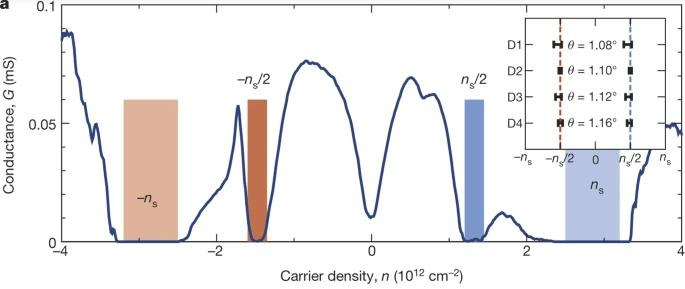
\includegraphics[width=\textwidth]{figures/ins.jpg}
		\caption{Measured conductance G of magic-angle twBLG device with $\theta=1.08^o$ and T = 0.3 K. The inset shows the density locations of half-filling states in the four different devices. Figure adapted from \cite{Cao2018}}
		\label{fig:ins}
	\end{subfigure}
	\begin{subfigure}{\linewidth}
		\centering
		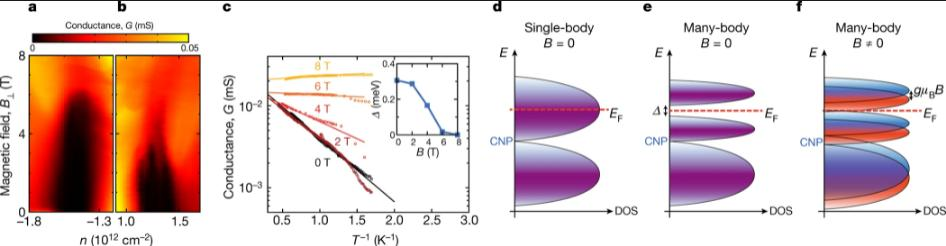
\includegraphics[width=\textwidth]{figures/mag.jpg}
		\caption{(a,b) Dependence of the conductance on the perpendicular magnetic field of the half-filling states. The measurement is taken at 0.3 K. (c) Arrhenius plot of the conductance of the p-side half-filling state at different magnetic fields. The inset shows the thermal activation gap. (d,e,f) Schematics of the density of states (DOS) in different scenarios, showing gap closing at non zero magnetic field. Figure adapted from \cite{Cao2018}}
		\label{fig:mag}
	\end{subfigure}
\end{figure}

They also found the presence of superconductivity states near the correlated insulating states. This can be seen from the temperature-carrier density phase diagram (fig. \ref{fig:sc}), which suggests a critical temperature upto 1.7 K. \cite{Cao2018_2} This is similar to phase diagrams with
superconductor states flanking Mott states in unconventional superconductors like cuprates. The superconductivity was confirmed by BKT phase transition in voltage–current power law
measurements, characteristic of 2D superconductors, and by phase-coherent transport behaviour from SQUID-like interference pattern (see fig \ref{fig:squid}). The temperature dependence of the perpendicular critical field is consistent with Ginzburg-Landau theory (see fig \ref{fig:glt}). The zero-temperature parallel critical magnetic field is larger than the value given by BCS theory, suggesting a possible unconventional origin of superconductivity.

\begin{figure}[H]
	\begin{subfigure}{\linewidth}
		\centering
		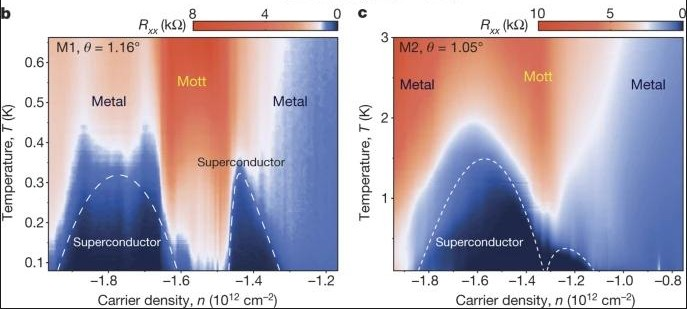
\includegraphics[width=0.8\textwidth]{figures/sc.jpg}
		\caption{Four-probe resistance versus temperature and carrier density for devices with twist angle (b) $1.16^o$ and (b) $1.05^o$. Two superconducting domes are observed next to the half-filling Mott state. Figure adapted from \cite{Cao2018_2}}
		\label{fig:sc}
	\end{subfigure}
	\begin{subfigure}{\linewidth}
		\centering
		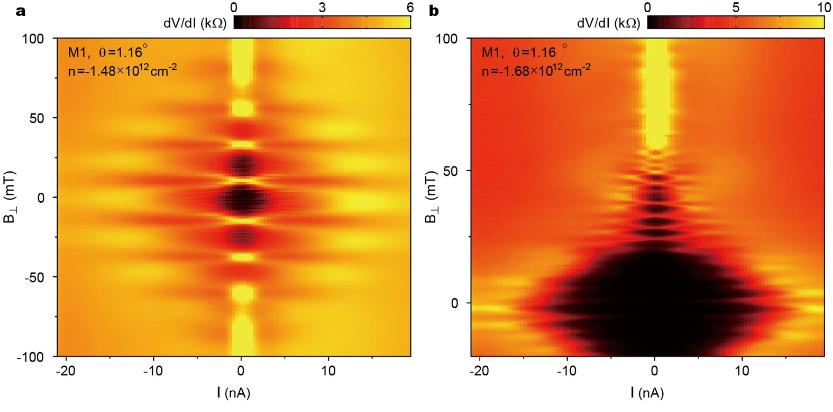
\includegraphics[width=0.8\textwidth]{figures/squid.jpg}
		\caption{Differential resistance dV/dI versus bias current and perpendicular field, at two different charge densities. Periodic oscillations are observed in the critical current. Figure adapted from \cite{Cao2018_2}}
		\label{fig:squid}
	\end{subfigure}
	\begin{subfigure}{\linewidth}
		\centering
		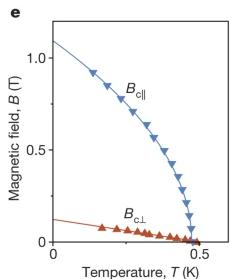
\includegraphics[width=0.4\textwidth]{figures/glt.jpg}
		\caption{Perpendicular and parallel critical magnetic field versus temperature. The fitting curves for perpendicular critical field correspond to Ginzburg–Landau theory for a two-dimensional superconductor. Parallel critical field is fitted to $B_{c\parallel}(0)(1-T/Tc)^{1/2}$. Figure adapted from \cite{Cao2018_2}}
		\label{fig:glt}
	\end{subfigure}
\end{figure}
Later, Xiaobo Lu and Dimitri Efetov
\textit{et al.} used mechanical squeezing process to improve the angle uniformity, and found resistance peaks at full filling ($v=4$), quarter ($v=1$), half ($v=2$) and three-quarter filling ($v=3$), i.e., correlated states developed
at all integer filling factors, which indicates a
full lift of the spin and valley degeneracies. \cite{Lu2019} The
observed superconductor domes appear not only at a doping
close to half filling, but also at around a quarter filling, with a
high critical temperature up to 3 K (see fig.\ref{fig:twBLG}).

\begin{figure}[H]
	\centering
	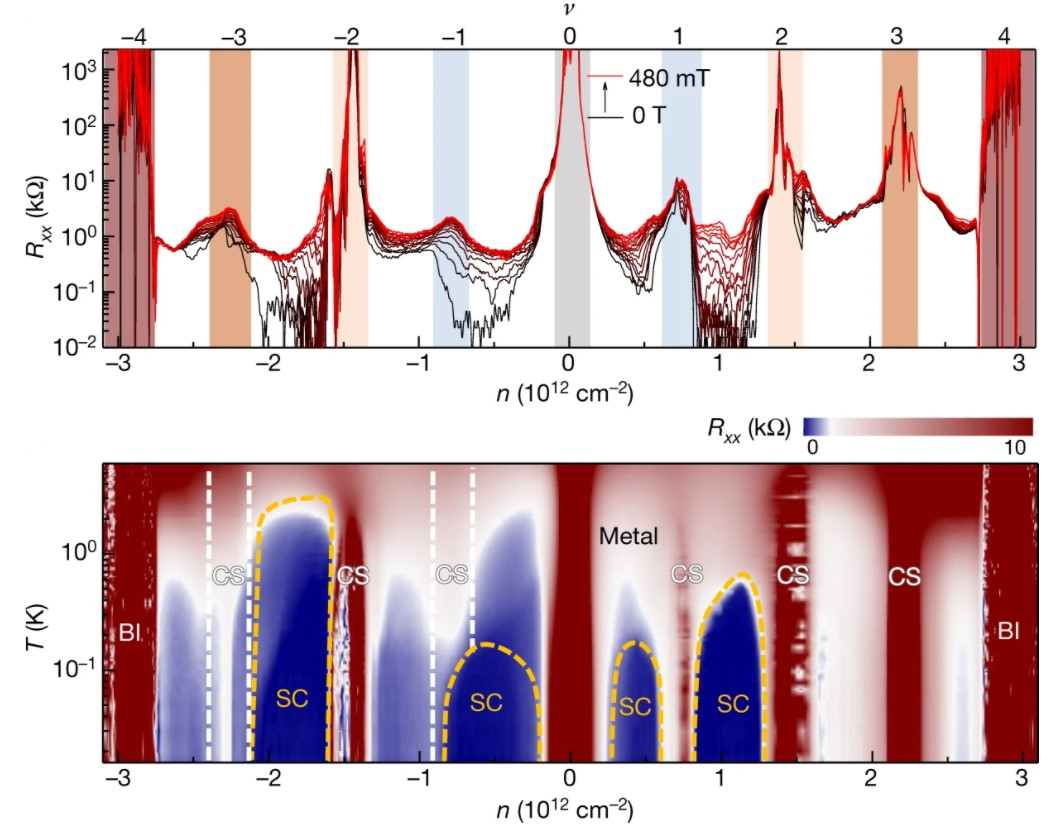
\includegraphics[width=0.8\textwidth]{figures/res_phase.jpg}
	\caption{twBLG transport signatures. Top:  Four-terminal longitudinal resistance plotted against carrier density at different perpendicular magnetic fields from 0 T (black trace) to 480 mT (red trace). Bottom:  Colour plot of longitudinal resistance against carrier density and temperature, showing different phases including metal, band insulator (BI), correlated state (CS) and superconducting state (SC). Figure adapted from \cite{Lu2019}}
	\label{fig:twBLG}
\end{figure}

The nature of superconductivity in twBLG is still an open question. On one hand, there are a number of similarities between the superconductor state in twBLG and unconventional superconductors: (1) Phase diagram in which superconductor accompanied by Mott insulator, \cite{Cao2018_2,Lu2019} similar to cuprates. (2) Linear-in-temperature resistance observed at higher temperature, \cite{Polshyn2019,str} similar to strange metal states in unconventional superconductor systems. On the other hand, there are experiments that suppress correlated insulator states, but keep the superconducting states, hinting at conventional superconductivity in twBLG. One way is by reducing the distance between twBLG and the gate, using thinner hBN dielectric layer, hence decreasing the correlation strength. \cite{Stepanov2020,Saito2020} Another way is by adding a tungsten-diselenide ($WSe_2$) on top of twBLG, which induces stronger spin–orbit interaction in twBLG, stabilising the superconducting state but closing gaps at all integer filling factors. \cite{Arora2020}

\begin{figure}[H]
	\centering
	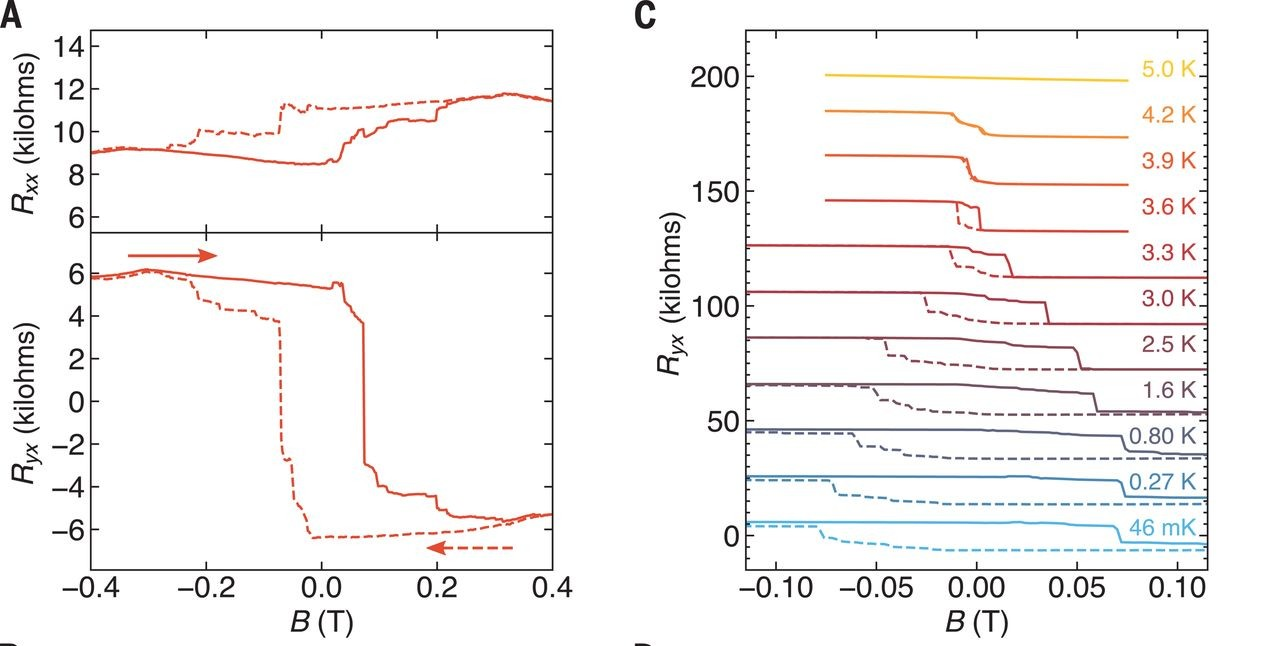
\includegraphics[width=\textwidth]{figures/ferro.jpg}
	\caption{(A) Magnetic field dependence of the longitudinal resistance $R_{xx}$ (upper panel) and Hall resistance $R_{yx}$ (lower panel) at 30 mK, showing a hysteretic AH effect resulting from emergent magnetic order. (C) Temperature dependence of $R_{yx}$ versus B between 46 mK and 5.0 K, showing the hysteresis loop closing with increasing temperature. Figure adapted from \cite{Sharpe605}}
	\label{fig:ferro}
\end{figure}

Another exciting and surprising discovery is the observation of ferromagnetism and quantum anomalous Hall effect (QAH) in twBLG. An emergent ferromagnetism near three-quarters filling of
the conduction Moiré band in twBLG was observed, with a giant zero-field
anomalous Hall signal and magneto hysteresis. \cite{Sharpe605} Later, well-developed quantum anomalous Hall effect with Chern number
C = 1 was confirmed. \cite{Serlin900} Since the twisted bilayer graphene is free of atomic magnetic moment, the counter-intuitive discovery of ferromagnetism \cite{Sharpe605} and
QAH \cite{Serlin900} is the result of a correlated Chern insulator. Aligning the bottom graphene layer and the hBN substrate gives rise to strong correlations of the Moiré band and gap opening, leading to the observed effects.

\begin{figure}[H]
	\centering
	\includegraphics[width=\textwidth]{figures/qah.jpg}
	\caption{(C) $R_{xy}$ as a function of B and n. The rear wall shows field-training symmetrized values of $R_{xy}$ at B = 0. Zero-field anomalous Hall signal becomes nonzero when ferromagnetism appears, and it reaches a plateau of $h/e^2$. (D) Schematic band structure at filling factors 4 and 3. The net Chern number is 1 at filling factor 3. Figure adapted from \cite{Serlin900}}
	\label{fig:qah}
\end{figure}

\section{Tunneling}
\label{section:t}
When the energy bands of two parallel 2D carrier systems are energetically aligned, momentum-conserving tunneling leads to a resonantly enhanced tunneling conductivity and negative differential resistance (NDR). Tutuc \textit{et al.} have worked on tunneling in graphene-insulator-graphene \cite{Mishchenko2014} and bilayer graphene-insulator-bilayer graphene. \cite{Tutuc,Tutuc17,Tutuc18} Fig. \ref{fig:bandov} shows the momentum shift caused due to twist between the two graphene layers in the graphene-hBN-graphene device. It also shows the alignment of the bands for different gate voltages. Fig. \ref{fig:single} shows the result of this band overlap. There is NDR and resonant tunneling seen. On application of in-plane magnetic field (see fig. \ref{fig:magtl}), there is an added momentum that changes band alignment and hence, resonant tunneling conditions.

\begin{figure}[H]
	\centering
	\includegraphics[width=0.5\textwidth]{figures/bandov.jpg}
	\caption{(a) Graphene-hBN-graphene device structure. (b) A rotation by $\theta$ of the two graphene layers in real space corresponds to the momentum shift $K_i^\pm$ between two Dirac points. (c,e,f) Relative alignment between the top (left cones) and bottom (right cones) graphene Dirac points. The boundary between magenta (empty states) and blue (filled states) marks the Fermi level. Figure adapted from \cite{Mishchenko2014}}
	\label{fig:bandov}
\end{figure}

\begin{figure}[H]
	\centering
	\includegraphics[width=0.4\textwidth]{figures/single.jpg}
	\caption{(a) Current density vs voltage curves at different gate voltages. (b) Conduction plots as a fuction of gate and bias voltage. Figure adapted from \cite{Mishchenko2014}}
	\label{fig:single}
\end{figure}

\begin{figure}[H]
	\centering
	\includegraphics[width=\textwidth]{figures/magtl.jpg}
	\caption{(b) Trajectories of the charged quasiparticles tunneling from top to bottom graphene layers in zero and finite magnetic fields caused by the Lorentz force. (c) dI/dV maps measured with a 15 T in-plane magnetic field applied. (e) Difference between the dI/dV maps with and without the in-plane magnetic field. Figure adapted from \cite{Mishchenko2014}}
	\label{fig:magtl}
\end{figure}

Moving on to bilayer graphene-insulator-bilayer graphene, it was seen that NDR still occurs and the tunneling conductivity is exponentially dependent on number of hBN layers (see \ref{fig:no}). Fig. \ref{fig:cons} shows that resonant tunneling occurs when charge neutrality points are aligned as it leads to maximum band overlap.

\begin{figure}[H]
	\centering
	\includegraphics[width=\textwidth]{figures/no.jpg}
	\caption{Interlayer current-voltage characteristics at (a) 10 K and (b) room temperature in double bilayer graphene - hBN. (c) Normalized	interlayer resistance vs number of hBN layers measured in multiple devices and at a low temperature of T = 1.4-20 K and at room temperature. Figure adapted from \cite{Tutuc}}
	\label{fig:no}
\end{figure}

\begin{figure}[H]
	\centering
	\includegraphics[width=\textwidth]{figures/cons.jpg}
	\caption{Energy band alignment and carrier densities at tunneling resonance in double bilayer graphene - hBN. (a) Energy band diagram of double bilayer graphene when charge neutrality points of top and bottom bilayers are aligned. (b) Interlayer bias vs back gate voltage at tunneling resonance (circles and squares) and when charge neutrality points are aligned (solid line) (c) Carrier densities of top and bottom layer at resonance tunneling. Figure adapted from \cite{Tutuc}}
	\label{fig:cons}
\end{figure}

Later, it was seen that there are two contributions to tunneling: one is unlike-band tunneling which happens when the overlap happens inside the chemical potential difference, other is like-band tunneling which happens when the bands are completely overlapped. The various possibleband alignments are shown in fig. \ref{fig:like}. Fig. \ref{fig:double} shows the same, but for tunneling conductivity. Based on the band alignment one can explain the changes in tunneling current at different gate and bias voltages.

\begin{figure}[H]
	\centering
	\includegraphics[width=\textwidth]{figures/like.jpg}
	\caption{Different contributions to the total interlayer tunneling current in double bilayer graphene - $WSe_2$. (a) Calculated interlayer tunneling current versus interlayer bias at top gate voltage -2 V and T = 1.5 K. The simulated data shows the total interlayer tunneling current (black), along with the like- (red) and unlike-band (green) tunneling. The symbols represent corresponding experimental data. (b) Energy band-alignment of the top (red) and bottom (green) graphene bilayers at various bias voltages. The dashed red (green) line marks the chemical potential of the top (bottom) graphene bilayer. Figure adapted from \cite{Tutuc17}}
	\label{fig:like}
\end{figure}

\begin{figure}[H]
	\centering
	\includegraphics[width=0.8\textwidth]{figures/double.jpg}
	\caption{Experimental (a) and calculated (b) interlayer conductivity vs interlayer bias and top gate voltage at back gate voltage -20 V and T = 1.5 K, in double bilayer graphene - $WSe_2$. The points labeled in (b) identify distinct tunneling regimes. (c) Energy band alignment of top (red) and bottom (blue) bilayer graphene bands corresponding to the biasing conditions labeled in (b). The dashed lines mark the two layer Fermi levels. Figure adapted from \cite{Tutuc18}}
	\label{fig:double}
\end{figure}

Now, looking at graphene-insulator-metal heterostructure, \cite{chaves2013model} the band diagram of a metal-graphene (MG) junction changes from isolated graphene and metal system at equilibrium, as shown in fig. \ref{fig:gim}. It forms a dipole layer as a result of charge transfer within the equilibrium separation distance. This is similar to having an insulator in between the junction. There is a potential difference $\Delta V$ due to the dipole/dielectric and a shift in fermi level of graphene, $\Delta E$. Fig. \ref{fig:gim2} shows various tunneling conditions, along with direction and magnitude of tunneling current. Applying a bias voltage V changes the relative difference between the Fermi levels on each side. If the Fermi level of graphene (metal) is above the fermi level of metal (graphene), tunneling current flows from graphene (metal) to metal (graphene). The magnitude of the tunneling current depends on the difference between the Fermi levels. In case of twBLG-insulator-metal, estimating the tunneling current isn't straight forward, as the band structure of twBLG is very different from that of graphene. Tunneling measurements are expected to provide insight into the band structure of twBLG, which is rich in electron correlation and has flat bands at magic angle.

\begin{figure}[H]
	\centering
	\includegraphics[width=0.8\textwidth]{figures/gim.jpg}
	\caption{(a) Band diagram of an isolated graphene and metal system. (b) Band diagram of a Metal-Graphene (MG) junction at equilibrium showing dipole formation at the	interface. (c) Nonequilibrium band diagram of the MG junction. Figure adapted from \cite{chaves2013model}}
	\label{fig:gim}
\end{figure}

\begin{figure}[H]
	\centering
	\includegraphics[width=0.8\textwidth]{figures/gim2.jpg}
	\caption{Schematic representation of the tunneling current between graphene and metal electrodes. Figure adapted from \cite{chaves2013model}}
	\label{fig:gim2}
\end{figure}
As we discussed earlier, in addition to conserving energy E, resonant tunneling between two parallel two-dimensional electron gases (2DEGs) requires the conservation of the in-plane momentum. Tunneling measurements help in the investigation of the broadening of the electronic states within an individual 2DEG, in a way that is not possible with conventional transport measurements. The lifetime broadening is characterized by the electron spectral function A($\mathbf k$,E), which describes the probability that an electron in a particular $\mathbf k$ state has energy E. A($\mathbf k$,E) is strongly peaked near the free-particle energy, with a width determined by the lifetime of the electron.

\begin{figure}[H]
	\centering
	\begin{subfigure}{.5\linewidth}
		\centering
		\includegraphics[width=\textwidth]{figures/tempdep.jpg}
		\caption{Temperature dependence of the equilibrium \\linewidth. The solid lines are fits to the \\form $a+bT^2$.}
		\label{fig:tempdep}
	\end{subfigure}%
	\begin{subfigure}{.5\linewidth}
		\centering
		\includegraphics[width=\textwidth]{figures/ndep.jpg}
		\caption{Log-log plot of the linewidth versus carrier density at T = 3 K.}
		\label{fig:ndep}
	\end{subfigure}
	\caption{Tunneling measurements done in devices with two GaAs quantum wells separated by a $Al_{0.33}Ga_{0.67}As$ barrier. Figure adapted from \cite{Ritchie}}
\end{figure}

Tunneling measurements done in devices with two modulation-doped GaAs quantum wells separated by a $Al_{0.33}Ga_{0.67}As$ barrier, \cite{Ritchie} show the density dependence of the electron-impurity scattering and the temperature dependence of the electron-electron scattering. Fig. \ref{fig:tempdep} shows the temperature dependence of the equilibrium linewidth. Only the electron-phonon and electron-electron scattering was expected to show significant temperature dependence. The temperature dependent component of the tunneling linewidth is due to electron-electron scattering as they saw a weak temperature dependence in sheet resistance. This indicates that the mobility is dominated by impurity sacttering and the temperature dependent electron-phonon contribution is small. It was observed that the linewidth exhibits an approximate $T^2$ temperature dependence coming from electron-electron scattering. Fig. \ref{fig:ndep} shows the carrier density dependence of the equilibrium linewidth. At low temperatures, the electron-electron scattering is negligible, and the tunneling linewidth is due to electron-impurity scattering. They see that the linewidth shows the power-law behavior expected ($\propto n^{-1/2}$) for small-angle scattering from remote ionized impurities.

Coming back to Graphene-hBN-metal heterostructures, signatures of phonon and defect-assisted tunneling have been observed. \cite{Chandni} They observe weak tunneling at low energies which is attributed to the absence of substantial overlap of the metal and graphene Fermi surfaces in momentum space. The enhancement in tunneling at higher energies is associated with the onset of inelastic processes in which phonons in the heterostructure provide the momentum necessary to overcome the Fermi surface mismatch. Fig. shows some of the possible phonon contributions to tunneling considering in-plane momentum conservation. An electron from a pole of the metal Fermi surface can use its out-of-plane momentum and a K-point phonon mode to tunnel on to the graphene Fermi Surface. An M-phonon mode can also contribute to the tunnel current since it can be shifted across the Brillouin zone to the K or $K^\prime$ point. This suggests that several phonons can contribute to tunneling by supplying appropriate out-of-plane momenta to the elecrons on the surface of the metal Fermi surface.

\begin{figure}[H]
	\centering
	\includegraphics[width=0.8\textwidth]{figures/phonon.jpg}
	\caption{Side-view of the Fermi surfaces of graphene and metal showing two possible phonon modes that contribute
		to tunneling. Figure adapted from \cite{Chandni}}
	\label{fig:phonon}
\end{figure}